\documentclass[]{article}
\usepackage{fontspec}
%\setmainfont{Arial}[ItalicFont={Arial Italic}]
%\setmainfont{Gill Sans MT}[ItalicFont={Gill Sans MT Italic}]
\usepackage[utf8]{inputenc}
\usepackage[margin=1.5cm, bindingoffset=1cm]{geometry}
\linespread{1.5}
\usepackage{float}
\usepackage{csquotes}
\usepackage{subfig}
\usepackage{graphicx}
\usepackage{wrapfig}
\usepackage{xcolor}
\usepackage{indentfirst}
\setlength{\parindent}{0cm}
\usepackage[italian]{babel}
\usepackage{amsmath,amssymb}
\usepackage{hyperref}
\usepackage{amsmath}
\usepackage{enumerate}
\usepackage{enumitem}
\setlist{nolistsep}
\setlist[enumerate]{align=left}
\setlist[itemize]{align=left}
% Imposto colore hyperlinks
\hypersetup{
    colorlinks=true,
    linkcolor=blue,
    urlcolor=blue,
    }
\usepackage{color}
\usepackage{listings}
\usepackage{wrapfig}
\usepackage{url}

\lstset{showstringspaces=false}

\title{CCFDetector}
\author{Marco Santoriello}
\date{Gennaio 2024}

\begin{document}
\begin{titlepage}
    \begin{center}
        \LARGE{\uppercase{Università degli Studi di Salerno}}\\
        \vspace{5mm}
        %Dipartimento
    	\uppercase{\normalsize Dipartimento di Informatica}\\
    \end{center}
    \begin{figure}[H]
        \centering
        
\includegraphics[width=0.35\textwidth]{img/logo_unisa.png}
    \end{figure}

    \begin{center}
        %Corso di Laurea
    	\normalsize{ Corso di Laurea in informatica }\\
    	\vspace{15mm}
    	%Titolo
        {\LARGE{\bf CCFDetector: Using ML against Credit Card Frauds }}\\
        {\large{ Progetto realizzato per l'esame di Fondamenti di Intelligenza Artificiale}}\\
    	\vspace{10mm}
    \end{center}
    \begin{minipage}[t]{0.4\textwidth}\raggedright
        %Candidato
    	{\large{Realizzato da: \\ \bf Marco Santoriello\\ Mat. 0512114100}}
    \end{minipage}

    \vspace{90mm}
    %Anno Accademico
    \centering{\large \uppercase{ Anno Accademico 2023/2024 }}

\end{titlepage}

\setcounter{tocdepth}{3} %IMPOSTO LIVELLO PROFONDITA' INDICE

\tableofcontents
\newpage


\section{Introduzione}
    Negli ultimi anni, sempre più piede hanno preso i pagamenti elettronici, al punto che, anche in Italia, per legge, ogni commerciante deve essere munito di un dispositivo che permetta al cliente di pagare utilizzando la propria carta di credito, rischiando, in caso di mancato adempimento a questa legge, ingenti sanzioni pecuniarie.\\
    Come è facile immaginare, questo cambiamento nel modo in cui il denaro viene messo in circolazione ha interessato notevolmente criminali e truffatori (i cosiddetti \textit{scammers}), i quali hanno trovato non pochi modi di impossessarsi illecitamente delle carte di credito altrui, o dei relativi dati associati ad esse.
    Basti pensare che negli Stati Uniti, secondo la \textit{Federal Trade Commission}, la tipologia di furto di identità più diffusa è proprio relativa alle frodi che interessano pagamenti elettronci.\\
    Queste frodi possono avvenire in svariati modi: si parte dal furto vero e proprio della carta di credito, fino ad arrivare, tramite diversi metodi, all'appropriazione dei soli dati della carta che abilitano al pagamento, passando per la clonazione delle carte e per l'utilizzo di dispositivi \textit{contactless} in posti affollati in prossimità dei portafogli delle ignare vittime.\\
    Questo progetto nasce con lo scopo di addestrare un modello di Machine Learning che permetta una facile ed affidabile individuazione delle transazioni fraudolente, con lo scopo di bloccarle tempestivamente per evitare sottrazioni di denaro alle vittime.
    Il progetto è consultabile nella sua interezza su \href{https://github.com/marcosantoriello/CCFDetector}{GitHub}.

    \subsection{Specifica PEAS}
        La specifica PEAS (Performance, Environment, Actuators, Sensors) è un sistema che permette di descrivere l'ambiente operativo di un agente intelligente. L'obiettivo principale del progetto è quello di massimizzare la capacità dell'agente di rilevare transazioni fraudolente. Di seguito la specifica PEAS:
        \begin{itemize}
            \item Performance: ROC-AUC Curve, precision, recall, f1.
            \item Environment: ambiente delle transazioni finanziarie.
            \item Actuators: algoritmo di classificazione.
            \item Sensors: dati ricevuti in input relativi ad una transazione.
        \end{itemize}

    \subsection{Caratteristiche dell'ambiente}
        L'ambiente operativo dell'agente risulta essere:
        \begin{itemize}
            \item \textbf{Single-agent}.
            \item \textbf{Completamente osservabile}: attraverso i sensori, l'agente godrà di una conoscenza completa dell'ambiente.
            \item \textbf{Dinamico}: l'ambiente delle transazioni finanziarie è in continua evoluzione. Di conseguenza lo sono anche i patterns relativi alle frodi.
            \item \textbf{Discreto}:le variabili assumono valori in un limitato intervallo; alcune, invece, assumono valori distinti e separati.
            \item \textbf{Episodico}: L'esperienza dell'agente è divisa in episodi atomici, dove ciascun episodio consiste dall'eseguire una singola azione.
            \item \textbf{Stocastico}: Lo stato dell'ambiente non è determinato dallo stato corrente o dall'azione eseguita dall'agente.
        \end{itemize}

    \subsection{Analisi del Problema}
        Il progetto mira, dunque, alla costruzione di un modello di Machine Learning, volto alla risoluzione di un problema di \textbf{apprendimento supervisionato}. In particolare, come verrà reso evidente da questo documento nelle successive sezioni, il problema da affrontare risulta essere di \textbf{classificazione binaria}, avendo da predire una variabile che puo' assumere valori 0, oppure 1.\\
        Gli strumenti utilizzati per la realizzazione sono elencati di seguito:
        \begin{itemize}
            \item \textbf{Python}.
            \item \textbf{Jupyter Notebook}.
            \item \textbf{PyCharm} come IDE.
            \item \textbf{LaTeX} per la documentazione.
            \item \textbf{Canva} per la presentazione.
            \item \textbf{GitHub} per il versioning.
        \end{itemize}

\section{Data Understanding}
    \subsection{Data Collection}
        Definito il Problem Statement, passo all'individuazione del dataset adatto per l'addestramento e la validazione del modello.\\
        Inizialmente sono partito da un \href{https://www.kaggle.com/datasets/mlg-ulb/creditcardfraud}{dataset reale} che, una volta addestrato non mi ha fornito i risultati sperati. Inoltre, tale dataset, vedeva nascosto il significato della maggior parte delle features, per ovvi motivi di privacy, rendendo il livello di explainability del modello molto basso. Da qui la scelta di ricorrere a dati simulati.
        La scelta è dunque ricaduta su un \href{https://www.kaggle.com/datasets/ealtman2019/credit-card-transactions/data}{dataset simulato} rilasciato da IBM.

    \subsection{Data Description}
        Il dataset in questione comprende dati, ottenuti attraverso un processo di simulazione che non è stato reso noto, di oltre 24 milioni di transazioni, di cui 30.000 fraudolente (cioè lo 0.1\%). Essendo dati simulati, ci si aspetta siano fedeli rappresentazioni delle transazioni reali e delle loro caratteristiche.\\
        Le features di questo dataset comprendono tutti i dettagli relativi a un pagamento elettronico (ID utente, ID carta, data, ora, modalità di pagamento, ecc.) e tutti i dettagli del venditore (i cui nomi sono stati codificati). La variabile target è rappresentata dalla colonna \textit{Is Fraud?}.\\
        Per ragioni legate alla capacità dell'hardware, decido di caricare soltanto 300.000 righe del dataset, verificando subito la presenza di transazioni fraudolente tra quelle importate.
        Procedo, a questo punto, con la documentazione dei dati.\\
        Il dataset contiene 15 colonne che riporto di seguito, associando ad ognuna una breve descrizione di essa:
        \begin{enumerate}[label=\roman*.]
            \item \textbf{User}: Id dell'utente che ha effettuato la transazione (Dtype: int64)
            \item \textbf{Card}: Id della carata che ha effettuato la transazione (Dtype: int64)
            \item \textbf{Year}: Anno in cui è avvenuta la transazione (Dtype: int64)
            \item \textbf{Month}: Mese in cui è avvenuta la transazione (Dtype: int64)
            \item \textbf{Day}: Giorno in cui è avvenuta la transazione (Dtype: int64)
            \item \textbf{Time}: Istante in cui è avvenuta la transazione (Dtype: object)
            \item \textbf{Amount}: Ammontare (in dollari) della transazione (Dtype: object)
            \item \textbf{Use Chip}: Modalità di pagamento (Dtype: object)
            \item \textbf{Merchant Name}: Nome del venditore presso cui si ha acquistato (Dtype: int64)
            \item \textbf{Merchant City}: Città del venditore presso cui si ha acquistato (Dtype: object)
            \item \textbf{Merchant State}: Stato del venditore presso cui si ha acquistato (Dtype: object)
            \item \textbf{Zip}: Zip code del venditore presso cui si ha acquistato (Dtype: float64)
            \item \textbf{MCC}: Merchant Category Code (Dtype: int64)
            \item \textbf{Errors?}: Se è avvenuto un errore, ne descrive la tipologia (Dtype: object)
            \item \textbf{Is Fraud?}: Transazione fraudolenta oppure lecita (Dtype: object)
        \end{enumerate}
        Per quanto riguarda le modalita' di pagamento, rappresentate nella colonna \textit{Use Chip}, osservo che sono di tre tipi:
        \begin{itemize}
            \item [-] \textit{Chip Transaction}: pagamento effettuato inserendo la carta, dotata di chip, nel lettore del terminale POS. Il chip, affinché la transazione possa essere autorizzata, richiede l'inserimento di un codice PIN.
            \item [-] \textit{Swipe Transaction}: pagamento effettuato utilizzando la striscia magnetica della carta. Tale tipologia di pagamento non prevede l'inserimento del PIN (perlomeno se il pagamento è al di sotto di una determinata soglia) per autorizzare la transazione.
            \item [-] \textit{Online Transaction}: pagamento online, effettuato inserendo i dati della carta manualmente, all'interno di un form. Anche in questo caso, a seconda dell'importo della transazione, potrebbe essere richiesta una misura di sicurezza aggiuntiva, oppure no.
        \end{itemize}
        Per poter continuare ad esplorare i dati, devo effettuare delle operazioni di conversione e splitting, anticipando, così, la fase di \textbf{data cleaning}.
        Innanzitutto, la feture \textit{Amount}, contenente l'importo di ogni transazione in dollari, non risulta essere in formato numerico, per cui vado a convertirne tutti i suoi valori in float, non prima di aver rimosso il simbolo della valuta che precede le cifre.\\
        Gestisco, poi, la caratteristica \textit{Time} che provvedo a dividere nelle caratteristiche \textit{Hour} e \textit{Minute}, rimuovendola, infine, dal dataset.
        Vado ora ad analizzare la distribuzione delle varie features, per cercare di capire meglio eventuali patterns legati con le frodi.\\
        In particolare, dal seguente grafico, osservo che la maggior parte degli importi che caratterizzano le transazioni fraudolente sono relativamente bassi, compresi, infatti nell'intervallo che va da 0 a 250 USD.
        \begin{figure}[H]
            \centering
            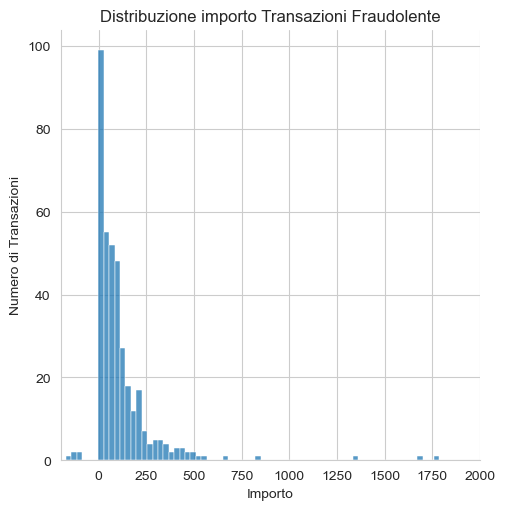
\includegraphics[width=.4\textwidth]{img/DistribuzioneImporto.png}
            \caption[short]{Distrubuzione degli importi relativi alle transazioni fraudolente}
        \end{figure}
        Inoltre, il metodo di pagamento maggiormente interessato da questo fenomeno, risulta essere il pagamento online. Invece, come mi aspettavo dalla precedente analisi fatta sui metodi di pagamento, quello tramite chip risulta essere il meno interessato, rivelandosi, dunque, il metodo piu' sicuro.
        \begin{figure}[H]
            \centering
            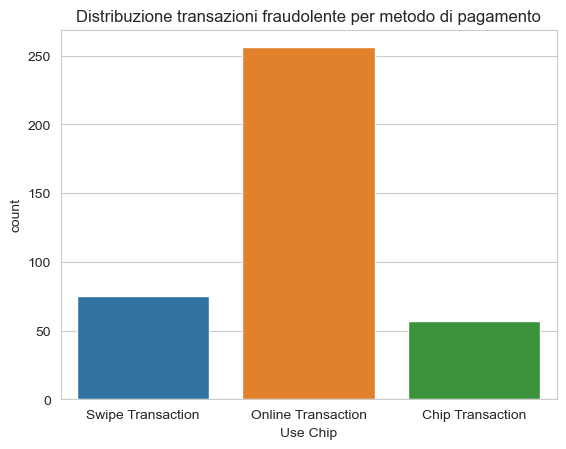
\includegraphics[width=.4\textwidth]{img/DistribuzioneMetodoPagamento.png}
            \caption[short]{Distribuzione dei metodi di pagamento}
        \end{figure}
        Infine, analizzando la distribuzione dei valori della categoria dei venditori, risulta che ci siano alcune categorie più soggette a frodi rispetto ad altre, come mostrato nel seguente grafico.
       \begin{figure}[H]
            \centering
            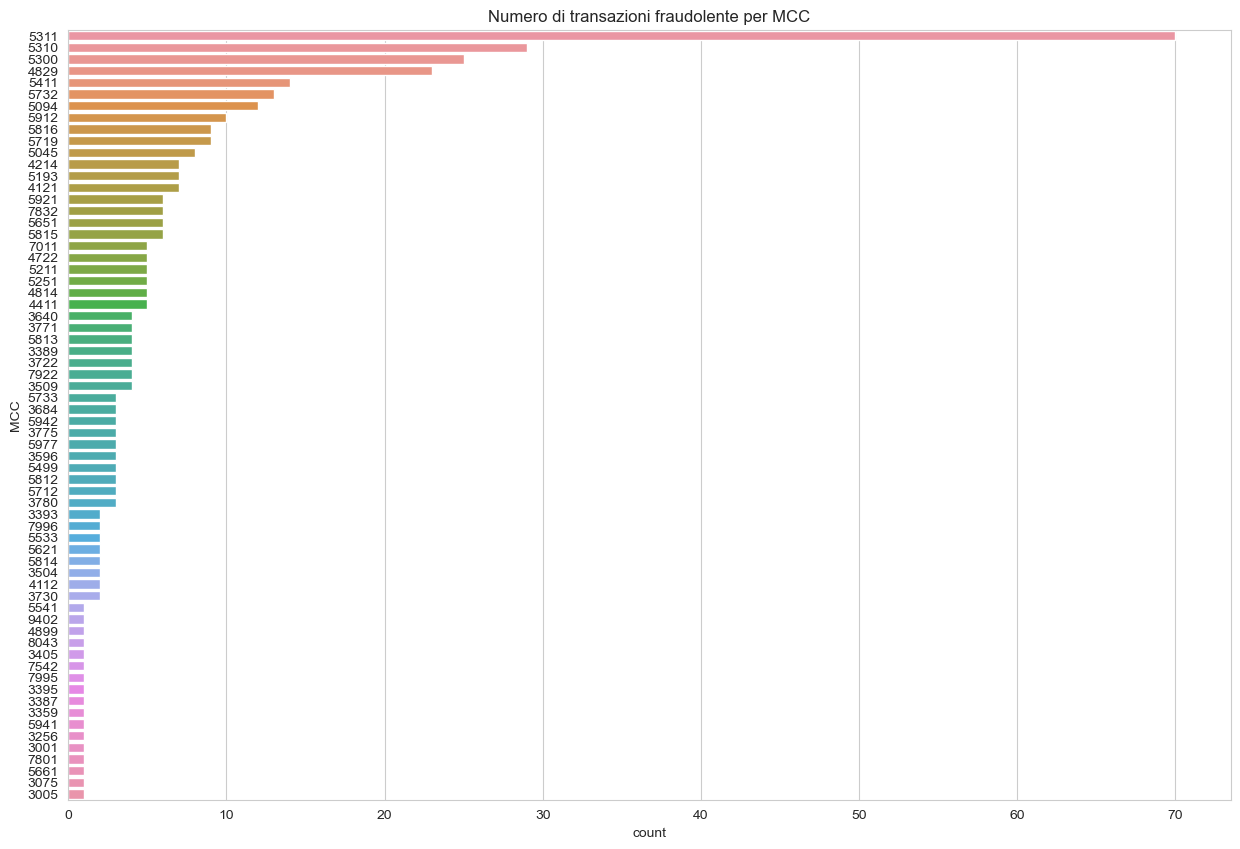
\includegraphics[width=.4\textwidth]{img/DistribuzioneMCC.png}
            \caption[short]{Distribuzione n. frodi per categoria di venditore}
        \end{figure}

    \subsection{Data Quality}
        Relativamente alla qualità dei dati, la prima cosa che noto è che le colonne \textit{Merchant State}, \textit{Zip}, ed, in particolare \textit{Errors}, contengono dei valori nulli.
        \begin{figure}[H]
            \centering
            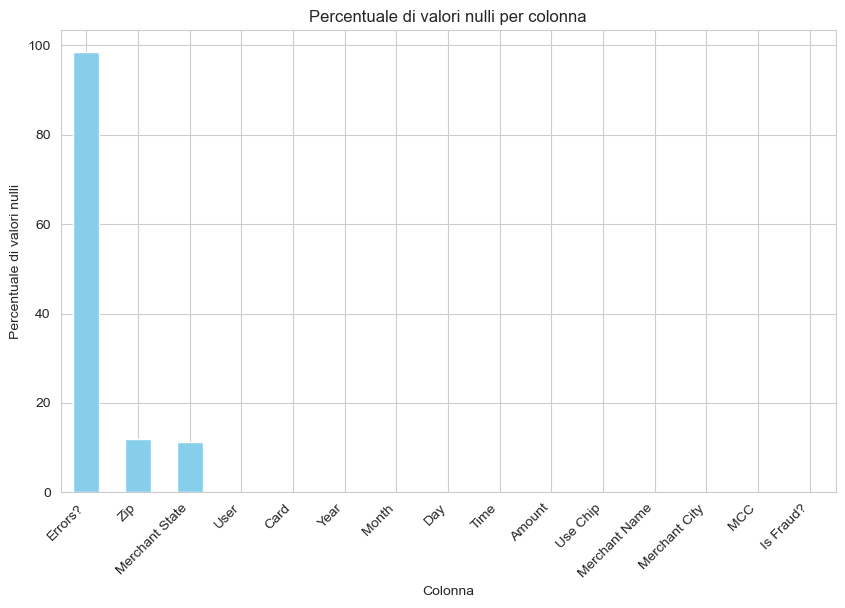
\includegraphics[width=.6\textwidth]{img/NullValuesPercentage.png}
            \caption[short]{Percentuale valori nulli per colonna}
        \end{figure}
        Inoltre, le caratteristiche \textit{Merchant State} e \textit{Zip} possono essere ricavate da \textit{Merchant City}, dunque potrebbe essere conveniente, contenendo valori nulli, rimuoverle.
        Procedo, dunque, a verificare è se il dataset è bilanciato o meno. Il numero di transazioni fraudolente è pari a 388, cioe' lo 0.129\% del totale delle transazioni. Il dataset risulta essere altamente sbilanciato, come mostrato dal seguente grafico:
        \begin{figure}[H]
            \centering
            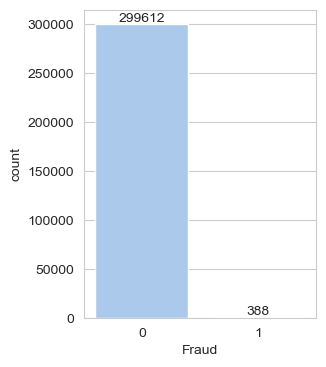
\includegraphics[width=.4\textwidth]{img/DistribuzioneFraudVsGen2.png}
            \caption[short]{Distrubuzione delle transazioni fraudolente e lecite}
        \end{figure}
        L’utilizzo di un dataset così sbilanciato, porterebbe alla costruzione di un modello altamente impreciso e che, probabilmente, si \textit{adatterà troppo} (\textit{overfitting}) al problema, in quanto andrebbe ad assumere la maggior parte delle transazioni come non fraudolente, siccome queste costituiscono la stragrande maggioranza dei dati.

\section{Data Preparation}
    In questa fase, vado ad effettuare le operazioni necessare per la pulizia dei dati, in modo che possano essere pronti per essere dati in input al modello.
    \subsection{Data Cleaning}
        Innanzitutto vado a gestire i valori nulli. Parto dalla caratteristica \textit{Errors?}. Come analizzato in fase di Data Understanding, questa colonna contiene le varie tipologie di errore a cui una transazione puo' andare incontro.
        Come risulta dall'osservazione dei valori di questa feature, i valori nulli sembrano corrispondere al caso in cui non si verifica alcun errore. Per tale ragione, decido di rimpiazzare tutti i valori nulli con il valore \textit{No error}. Tale modo di gestire i valori nulli si definisce \textbf{imputazione deduttiva}.\\
        Come secondo step, vado a rimuovere le colonne \textit{Merchant State} e \textit{Zip}. Esse, infatti, posso essere ricavate dalla feature \textit{Merchant City}, per cui, contenendo specialmente dei valori nulli, risulta conveniente la loro rimozione dal dataset.\\
        Necessitando per il futuro addestramento del modello di dati numerici, vado a convertire le variabili categoriche \textit{Use Chip}, \textit{Merchant City} ed \textit{Errors} in variabili numeriche, utilizzando il metodo \textbf{LabelEncoder()}, della libreria \textit{scikit-learn}. Tale metodo assegna un intero univoco ad ogni categoria, in ordine di scoperta.
    \subsection{Feature Scaling}
        Nella fase di Feature Scaling, proseguo con l'osservazione delle distribuzioni dei valori delle varie caratteristiche, poiché addestrare un modello su un dataset che contiene colonne con insiemi di valori molto diversi tra loro, potrebbe portare tale modello a confondersi, sovrastimando o sottostimando l'importanza delle varie caratteristiche.\\
        Le varie features, tra loro, assumono valori compresi in diversi ranges, per tale ragione, decido di effettuare la normalizzazione su tutte, tranne che sulla variabile dipendente.\\
        Per lo scopo, utilizzo la tecnica di \textbf{Normalizzazione min-max}, che è una delle più comuni e diffuse tecniche di normalizzazione.
        Di seguito riportata la formula della Normalizzazione min-max:
        \begin{center}
            \[
                x_{\text{norm}} = a + \frac{{x - \min(X)}}{{\max(X) - \min(X)}} \cdot (b - a)
            \]
        \end{center}
        Normalizzati i valori, passo alla fase di Feature Selection.

    \subsection{Feature Selection}
        Procedo con la fase di Feature Selection, in cui, come suggerisce il nome, vado ad individuare e selezionare le features che hanno potenza predittiva più alta, scartando quelle con potenza predittiva più bassa. Infatti, queste ultime potrebbero rendere il futuro modello più impreciso o peggiorarne le perfomances.\\
        La tecnica che utilizzo è nota come \textbf{Matrice di Correlazione} (senza escludere la possibilità di integrare l'analisi con le osservazioni fatte in fase di data exploration). Tale matrice mostra i \textit{coefficienti di correlazione} tra coppie di variabili. I coefficienti possono assumere valori nell'intervallo [-1, 1]. Valori vicini a 1 indicano che le due variabili sono \textbf{correlate positivamente}; valori vicini a -1 indicano che le due variabili sono \textbf{correlate negativamente}; valori vicini a 0, infine, indicano che tra le due variabili \textbf{non itercorre alcuna relazione}.
        \begin{figure}[H]
            \centering
            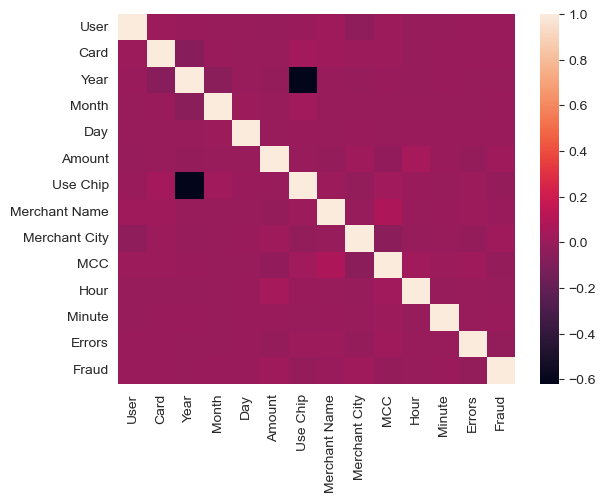
\includegraphics[width=.6\textwidth]{img/CorrelationMatrix.png}
            \caption[short]{Matrice di correlazione}
        \end{figure}
        Per avere una rappresentazione ancora più chiara, vado a mostrare solo il grado di relazione che ciascuna variabile ha con la variabile dipendente.
        \begin{figure}[H]
            \centering
            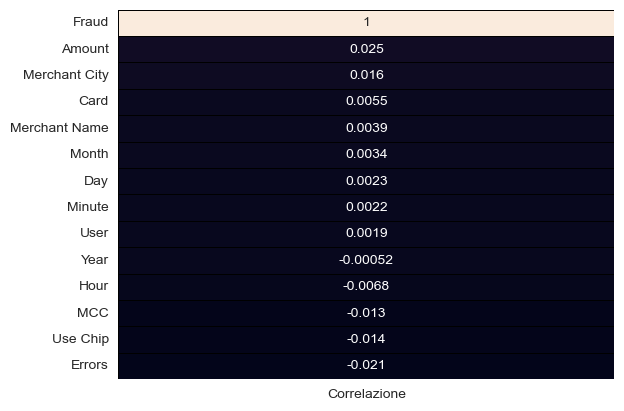
\includegraphics[width=.5\textwidth]{img/Correlation.png}
            \caption[short]{Correlazione tra features e variabile target}
        \end{figure}
        Le variabili maggiormente correlate con il target sono:
        \begin{itemize}
            \item [-] \textit{Amount}
            \item [-] \textit{Merchant City}
            \item [-] \textit{MCC}
            \item [-] \textit{Use Chip}
            \item [-] \textit{Errors}
        \end{itemize}
        Dunque, vado a scartare le restanti features, ad eccezione di \textit{Hour}, poiché, come precedentemente analizzato, sembrano esserci delle fasce orarie particolarmente interessate da attività fraudolente.
    \subsection{Data Balancing}
        Come analizzato nella fase di Data Understanding, il dataset risulta essere altamente \textit{unbalanced}. Addestrare un modello su un dataset del genere, comporterebbe un elevato rischio di overfitting. Per ridurlo, è necessario andare a bilanciare il dataset.
        \subsubsection{Sampling Techniqe Selection}
            Per bilanciare un dataset, posso utilizzare principalmente due tecniche (nelle varie declinaizoni):
            \begin{itemize}
                \item \textbf{undersampling},
                \item \textbf{oversampling}.
            \end{itemize}
            La tecnica di undersampling, in generale, consiste nella rimozione di samples dalla classe di maggioranza che, nel nostro caso, è quella delle transazioni non fraudolente. Tuttavia, scegliendo di utilizzare questa tecnica, mi ritroverei con un dataset eccessivamente piccolo, che vedrebbe perdute la maggior parte delle informazioni, avendo soltanto, come osservato in precedenza, 388 samples della classe di minoranza (Frauds).\\
            Allo stesso tempo, la tecnica di oversampling, che, invece, consiste nella generazione casuale di nuovi samples della classe di minoranza, potrebbe condurre il modello verso l'overfitting, in quanto, ancora, il numero dei samples della classe di minoranza e' eccessivamente basso.\\
            Per tale ragione, decido di utilizzare una tecnica nota come \textbf{Synthetic Minority Oversampling Tecnhique} (\textbf{SMOTE}).
            SMOTE e' una tecnica di oversampling che, invece di creare copie di istanze esistenti della classe di minoranza, genera nuove istanze (dette istanze sintetiche) attraverso l'interpolazion. Dunque, mi permette di mitigare il rischio di overfitting. Di seguito illustrato il funzionamento:
            \begin{enumerate}
                \item Seleziona una istanza random all'interno della classe di minoranza
                \item Identifica k vicini per il dato appena selezionato
                \item Seleziona uno di questi vicini per il nuovo dato da creare
                \item Calcola la distanza vettoriale tra il punto e il vicino selezionati
                \item Moltiplica tale distanza per un numero casuale compreso tra 0 e 1
            \end{enumerate}
            \begin{figure}[H]
                \centering
                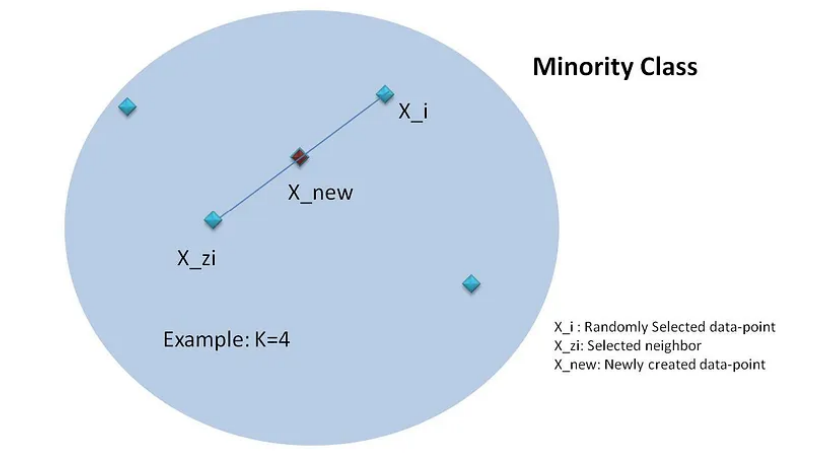
\includegraphics[width=.45\textwidth]{img/SMOTE.png}
                \caption[short]{Meccanismo SMOTE}
            \end{figure}
            Prima dell'applicazione di SMOTE, all'interno dei dati di training si hanno:
            \begin{itemize}
                \item N. transazioni fraudolente: 388
                \item N. transazioni non fraudolente: 299612
            \end{itemize}
            Dopo l'applicazione di SMOTE, invece, si hanno:
            \begin{itemize}
                \item N. transazioni fraudolente: 299612
                \item N. transazioni non fraudolente: 299612
            \end{itemize}

\section{Data Modeling}
    Prima di proceder con l'addestramento del modello, divido il dataset in \textit{training set} e \textit{test set}. E' cruciale effettuare questa divisione prima dell'addestramento del modello per evitare di incappare in problemi di \textbf{data leakage}. Infatti, sarebbe un errore testare e valutare il modello sugli stessi dati. Se così non fosse, infatti, il modello effettuerebbe predizioni accurate in fase di addestramento, ma non in fase di rilascio.\\
    Dunque, innanzitutto separo le features dalla variabile target. Per fare questo, utilizzo il metodo \textit{iloc} della libreria pandas: in particolare, nella prima istruzione seleziono tutte le righe, tramite \textit{:}, delle prime sette colonne (da 0 a 6) e poi, tramite \textit{values}, converto in un array numpy; nella seconda istruzione, invece, seleziono tutte le righe della ottava colonna (di indice 7)  del dataframe.
    \begin{verbatim}
        # Separating features and target
        X = df1.iloc[:,:7].values
        y = df1.iloc[:,7].values
    \end{verbatim}
    Successivamente, divido il dataset assegnando il 30\% dei dati al test set, mentre il restante 70\% di essi costituiranno i dati di addestramento.
    \subsubsection{Classificatori}
        Avendo di fronte un problema di classificazione binaria, vari sono gli algoritmi utilizzabili per addestrare il modello. Per gli scopi di questo progetto, decido di utilizzare le conoscenze acquisite durante il corso di FIA, scegliendo l'algoritmo \textbf{Naive Bayes} e riprendendo l'algoritmo \textbf{Decision Tree}, applicato, però, nel contesto dell'\textit{Ensemble Learning}, cioè utilizzerò il classificatore \textbf{Random Forest}.
        \subsubsection{Naive Bayes}
            Naive Bayes è un algoritmo di classificazione che, date le caratteristiche di una nuova istanza da classificare, calcola le probabilità che queste facciano parte di una classe tramite l'appilicazione del \textit{teorema di Bayes}. L'algoritmo viene chiamato \textit{naive} poiché non considera le correlazioni che ci sono tra le varie caratteristiche, supponendo che ognuna di esse sia indipendente dall'altra. Di seguito riportato il teorema sopracitato:
            \begin{center}
            \[
                P(A|B) = \frac{P(B|A) \cdot P(A)}{P(B)}
            \]
        \end{center}
        Esistono tre varianti di Naive Bayes:
        \begin{itemize}
            \item \textbf{Gaussian Naive Bayes}: adatto quando i dati sono disposti secondo una distribuzione gaussiana.
            \item \textbf{Bernoulli Naive Bayes}: adatto quando i dati sono disposti secondo una distribuzione di Bernoulli.
            \item \textbf{Multinomial Naive Bayes}: adatto quando i dati sono disposti secondo una distribuzione multinomiale.
        \end{itemize}
        Per scegliere quale delle tre varianti, eventualmente, utilizzare, decido di addestrare tre modelli diversi e confrontare le loro prestazioni, utilizzando una matrice di confusione.
        \begin{figure}[H]
            \centering
            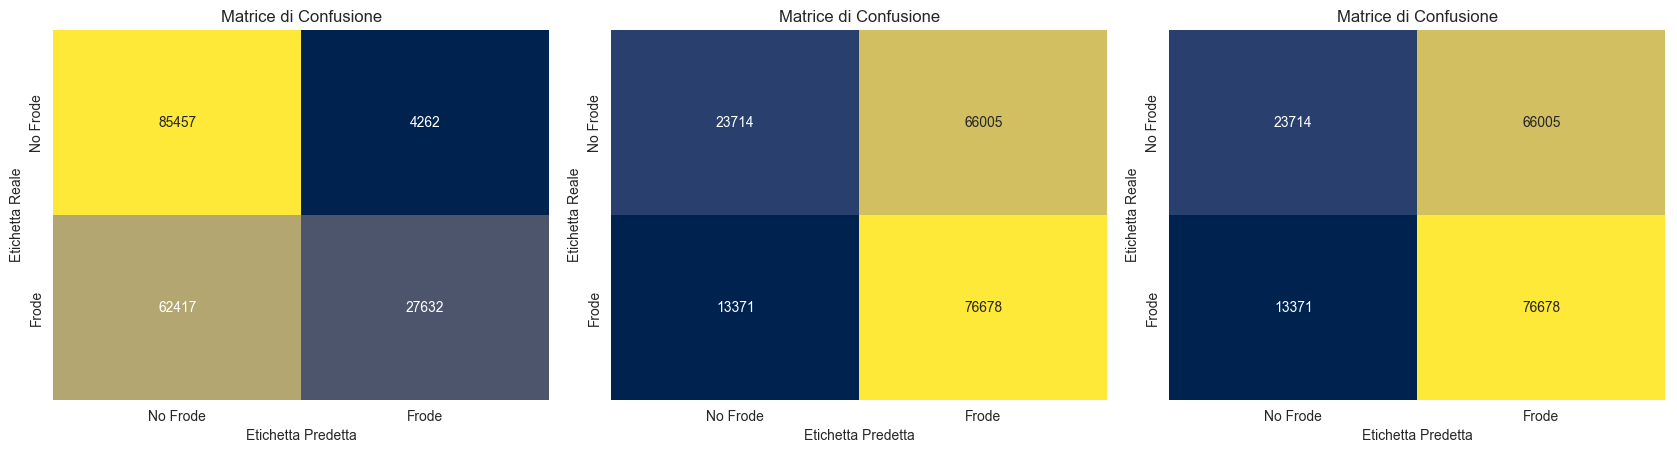
\includegraphics[width=1\textwidth]{img/ConfrontoMatrici.png}
            \caption[short]{Matrici di confusione - Varianti Naive Bayes}
        \end{figure}
        Dalle matrici di correlazione appena visualizzate, posso ricavare le seguenti metriche:
        \begin{itemize}
            \item \textbf{Accuracy}: indica il numero totale di predizioni corrette (considera sia i True positives che i True negatives).
            \item \textbf{Precision}: indica il numero di predizioni corrette per la classe \textit{True} rispetto al totale delle predizioni effettuate dal modello.
            \item \textbf{Recall}: indica il numero di predizioni corrette per la classe \textit{True} rispetto a tutte le istanze positive di quella classe. Indica, cioè quante istanze positive riesce ad individuare.
        \end{itemize}
        Sottolineo che, in presenza di dataset fortemente sbilanciati, l'accuracy non è una metrica particolarmente affidabile, in quanto assumerebbe un valore alto poiché predirebbe con facilità la maggior parte dei valori della classe di maggioranza. Tuttavia, in questo caso, avendo precedentemente bilanciato il dataset, posso utilizzarla senza troppi problemi. Anche se il \textbf{recall} è la metrica che intendo massimizzare in quanto voglio essere sicuro di rilevare il maggior numero di transazioni fraudolente, anche a costo di etichettare come fraudolenta qualche transazione che in realtà è lecita (che verrebbe successivamente autorizzata in seguito ad ulteriori verifiche da parte del carholder).\\
        A questo punto, analizzo le metriche ottenute dai vari classificatori.
        \begin{center}
        \begin{tabular}{|c|c|c|c|}
            \hline
            \textbf{Classificatore} & \textbf{Accuracy} & \textbf{Precision} & \textbf{Recall}\\ \hline
            Gaussian NB & 0.6290830403631347 & 0.8663698501285508 & 0.30685515663694213 \\ \hline
            Bernoulli NB & 0.5584531173512527 & 0.537401091931064 & 0.8515141756154982 \\ \hline
            Multinomial NB & 0.5584531173512527 & 0.537401091931064 & 0.8515141756154982 \\ \hline
        \end{tabular}
    \end{center}
    Bernoulli Naive Bayes e Multinomial Naive Bayes, sono quelli che danno migliori risultati in termini di Recall, a discapito di Precision e Accuracy. Infatti, questi due algoritmi riescono ad identificare un numero elevato di transazioni fraudolente, ma allo stesso tempo classificano molte transazioni lecite come fraudolente (Falsi Positivi).
    \subsubsection{Random Forest}
        A questo punto addestro il classificatore \textbf{Random Forest}. Tale algoritmo, combina l'output di più strutture (Ensemble Learning) ad \textit{albero decisionale} per raggiungere un unico risultato. Ricordo che il \textbf{Decision Tree} è un classificatore che cerca il modo migliore (sulla base dell'information gain di una features, che a sua volta è basato su entropia) per suddividere i dati. Random Forest combina i risultati di più alberi decisionali fornendo, generalmente, risultati più accurati.\\
        Di seguito riporto la Confusion Matrix del modello basato su Random Forest e le metriche da essa derivanti.
        \begin{figure}[H]
            \centering
            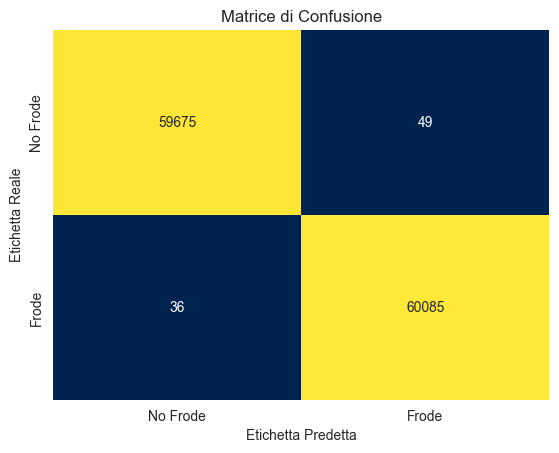
\includegraphics[width=.55\textwidth]{img/RFMatrix.png}
            \caption[short]{Matrici di confusione - Random Forest}
        \end{figure}
        Risultati:
        \begin{itemize}
            \item \textbf{Accuracy}: 0.9974689599928798
            \item \textbf{Precision}: 0.9968390932079322
            \item \textbf{Recall}: 0.9981121389465736
        \end{itemize}
        E' già evidente la qualità superiore di questo modello, che ha prodotto risultati molto soddisfacenti. Nella seguente tabella, riassumo tutti i risultati ottenuti.
        \begin{center}
        \begin{tabular}{|c|c|c|c|}
            \hline
            \textbf{Classificatore} & \textbf{Accuracy} & \textbf{Precision} & \textbf{Recall}\\ \hline
            Gaussian NB & 0.6290830403631347 & 0.8663698501285508 & 0.30685515663694213 \\ \hline
            Bernoulli NB & 0.5584531173512527 & 0.537401091931064 & 0.8515141756154982 \\ \hline
            Multinomial NB & 0.5584531173512527 & 0.537401091931064 & 0.8515141756154982 \\ \hline
            Random Forest & 0.9974689599928798 & 0.9968390932079322 & 0.9981121389465736 \\ \hline
        \end{tabular}
    \end{center}
    Il classificatore che scelgo, dunque è il \textbf{Random Forest}.
\section{Evalutation}
    A questo punto, vado ad analizzare la curva ROC del modello scelto.\\
    Una curva ROC (Receiver Operator Characteristic) misura l'accuratezza di un classificatore binario per tutto l'intervallo di valori. Tale curva viene creata tracciando il valore del \textit{True Positive Rate} (asse y) rispetto al \textit{False Positive Rate} (asse x). Il punto di coordinate (0, 1) rappresenta il punto ideale: più la curva gli si avvicina, migliore è la qualità delle sue predizioni. Dalla curva ROC, possiamo studiare l'\textit{Area Under the Curve} (AUC). Un classificatore per cui risulta $AUC=1$ è l'ideale poiché vuol dire che riesce a cogliere perfettamente la distinzione tra le classi dei Positivi e dei Negativi.
    Il classificatore prima implementato, restituisce $AUC=1$, dunque è davvero soddisfacente.
    \begin{figure}[H]
            \centering
            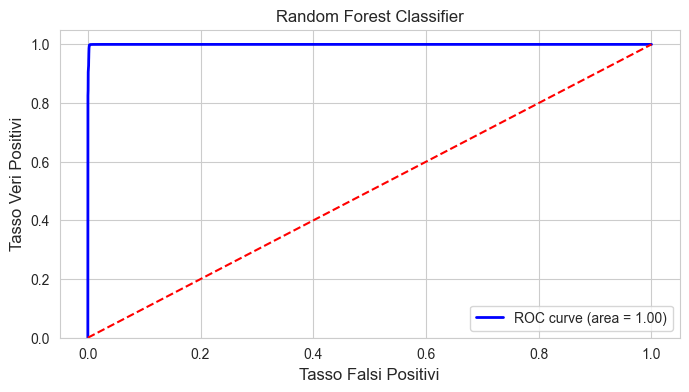
\includegraphics[width=.55\textwidth]{img/RF-ROC-AUC.png}
            \caption[short]{ROC-AUC per il modello addestrato}
    \end{figure}
    Per completare le osservazioni effettuate in fase di Data Understanding, attraverso un'ulteriore analisi del modello, sono andato a ricavare le features che più risultano essere correlate a transazioni fraudolente e sono riportate nel seguente grafico:
    \begin{figure}[H]
            \centering
            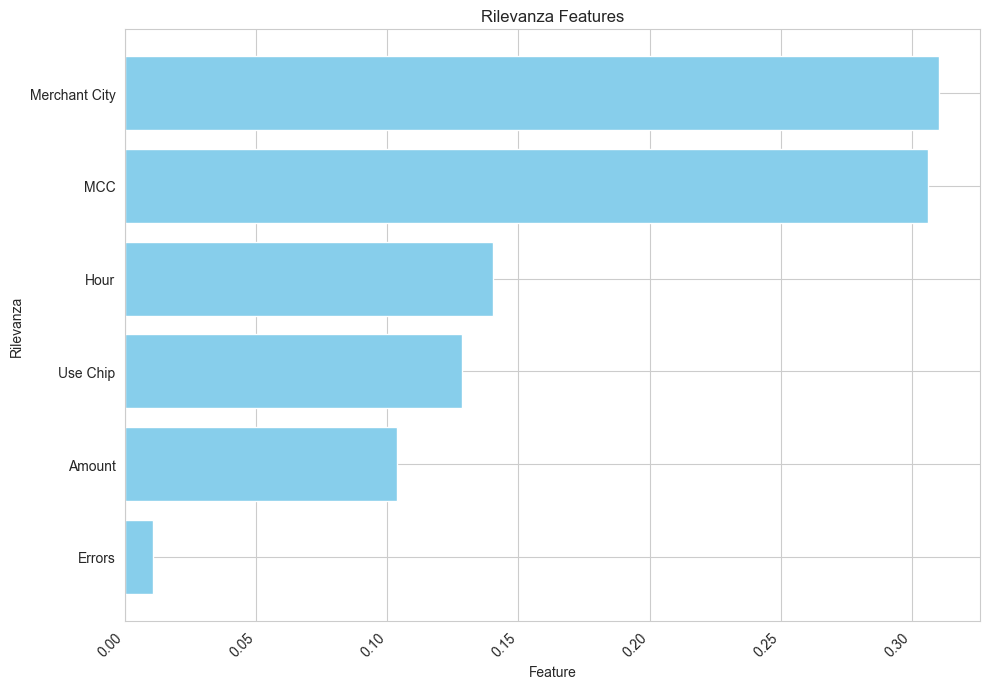
\includegraphics[width=.65\textwidth]{img/RilevanzaFeatures.png}
            \caption[short]{Features maggiormente correlate a casi di frode}
    \end{figure}
    Come si osserva, la posizione del venditore è particolarmente rilevante, così come la sua categoria di business. Osserviamo, inoltre, che ci sono fasce orarie particolarmente interessate da attività fraudolente. \\

\section{Conclusioni}
    Questo progetto è stato realizzato come prova di esame per l'esame di Fondamenti di Intelligenza Artificiale. Grazie ad esso ho avuto la possibilità di approfondire tutte le fasi dello sviluppo di un sistema di Machine Learning (ho seguito il modello CRISP-DM), integrando le conoscenze acquisite durante il corso, con nuove conoscenze in seguito a varie ricerche.\\
    \subsection{Sviluppi Futuri}
        Il modello non nasce per essere utilizzato da utenti comuni, bensì dovrebbe essere integrato da un sistema più grande, dal quale passano le transazioni effettuate in tempo reale per decidere se bloccarla oppure no.\\
\end{document}